
\section{Tổng quan về kiến trúc hệ thống}

    \hspace*{0.8cm}Kiến trúc hệ thống là nền tảng quan trọng trong phát triển ứng dụng di động, nơi các thành phần như thiết bị, ứng dụng và server phối hợp hoạt động. Trong phần này, người đọc sẽ tìm hiểu về vai trò của kiến trúc trong việc đảm bảo hiệu suất, khả năng mở rộng và tính ổn định của ứng dụng. Các yếu tố như tính đồng nhất, tính trong suốt và tính khả chuyển sẽ được trình bày như những tiêu chí thiết kế quan trọng. Bên cạnh đó, những mô hình kiến trúc phổ biến và công nghệ hỗ trợ như microservices, containerization, cùng các công cụ DevOps sẽ giúp hình dung rõ hơn về cách xây dựng một hệ thống di động hiện đại và hiệu quả.

    % 1.1.
    \subsection{Tổng quan về kiến trúc hệ thống trong ứng dụng di động}
    \renewcommand{\labelitemi}{--}    
    
    \hspace*{0.8cm}Kiến trúc hệ thống trong phát triển ứng dụng di động là nền tảng kỹ thuật bao gồm ba thành phần chính: phần cứng thiết bị, ứng dụng di động và hệ thống server hỗ trợ phía sau. Mục tiêu chính của kiến trúc này là thiết lập một hệ thống có khả năng vận hành đồng nhất, đảm bảo tính trong suốt giữa các thành phần và đạt được mức độ khả chuyển cao.
    
    \vspace{0.5em}
  
    \hspace*{0.8cm}Việc xây dựng kiến trúc hệ thống hợp lý đóng vai trò quan trọng đối với sự thành công của một ứng dụng. Trước hết, kiến trúc hệ thống ảnh hưởng trực tiếp đến hiệu suất hoạt động cũng như khả năng mở rộng trong tương lai. Bên cạnh đó, một kiến trúc ổn định sẽ giúp ứng dụng hoạt động mượt mà và hạn chế lỗi phát sinh trong quá trình sử dụng. Quan trọng hơn, khi các thành phần trong hệ thống được tổ chức rõ ràng, việc phát hiện và xử lý lỗi sẽ trở nên nhanh chóng và chính xác hơn.
    

    % 1.2.
    \subsection{Các yếu tố quan trọng trong kiến trúc hệ thống}
    \renewcommand{\labelitemi}{--}
    
        \hspace*{0.8cm}Một kiến trúc hệ thống hiệu quả cần đảm bảo ba yếu tố cốt lõi: tính đồng nhất, tính trong suốt và tính khả chuyển.
    
        \vspace{0.5em}
    
        \hspace*{0.8cm}Tính đồng nhất là yêu cầu đầu tiên đối với một hệ thống hiện đại. Để đảm bảo sự nhất quán về dữ liệu giữa client và server, các kiến trúc sư phần mềm thường sử dụng các giao thức và tiêu chuẩn truyền thông như RESTful API hoặc GraphQL \cite{restgraphql}. Các chuẩn này không chỉ hỗ trợ chuẩn hóa quá trình giao tiếp giữa các thành phần mà còn giúp quản lý dữ liệu được lưu trữ và đồng bộ hóa một cách chính xác và hiệu quả trong toàn hệ thống.
      
        \vspace{0.5em}
      
        \hspace*{0.8cm}Tính trong suốt đóng vai trò thiết yếu trong việc phát hiện và xử lý lỗi. Một hệ thống được thiết kế tốt cần có khả năng ghi nhận và thông báo lỗi một cách rõ ràng. Để đạt được điều này, các công cụ như Firebase Crashlytics hoặc Sentry thường được tích hợp vào quá trình vận hành nhằm hỗ trợ theo dõi sự cố theo thời gian thực \cite{firebasecrashlytics}. Đồng thời, kiến trúc hệ thống cũng cần hỗ trợ việc kiểm tra và sửa lỗi một cách nhanh chóng, đảm bảo giảm thiểu gián đoạn trong quá trình vận hành.
      
        \vspace{0.5em}
      
        \hspace*{0.8cm}Tính khả chuyển đề cập đến mức độ linh hoạt của hệ thống khi có sự thay đổi về công nghệ hoặc thành phần. Trong kiến trúc hiện đại, việc áp dụng mô hình microservices hoặc modular architecture cho phép chia tách các thành phần độc lập, từ đó giúp việc thay thế hay nâng cấp trở nên dễ dàng mà không gây ảnh hưởng đến toàn hệ thống \cite{microservices}. Ngoài ra, công nghệ containerization như Docker hoặc Kubernetes cũng được sử dụng phổ biến nhằm tăng khả năng triển khai linh hoạt và đồng nhất giữa các môi trường khác nhau.
      

    % 1.3.
    \subsection{Các mô hình kiến trúc phổ biến trong ứng dụng di động}
    \renewcommand{\labelitemi}{--}
    
        \hspace*{0.8cm}Hiện nay, trong phát triển ứng dụng di động, có một số mô hình kiến trúc được sử dụng phổ biến nhằm đảm bảo tính tổ chức và hiệu quả trong vận hành.
    
        \vspace{0.5em}
    
        \hspace*{0.8cm}Mô hình Layers (hay kiến trúc ba lớp) là một cách tiếp cận cơ bản, trong đó ứng dụng được chia thành ba thành phần: lớp giao diện người dùng (UI), lớp xử lý nghiệp vụ (Business Logic), và lớp dữ liệu (Data). Cách chia lớp rõ ràng này giúp tách biệt các chức năng, tạo điều kiện thuận lợi cho việc bảo trì và mở rộng ứng dụng.
      
        \vspace{0.5em}
      
        \hspace*{0.8cm}Một mô hình quen thuộc khác là MVC (Model-View-Controller), trong đó phần dữ liệu và logic được tách biệt rõ ràng với giao diện và phần xử lý sự kiện. Model chịu trách nhiệm quản lý dữ liệu và logic nghiệp vụ, View đảm nhiệm việc hiển thị giao diện, còn Controller xử lý các hành động của người dùng và điều phối tương tác giữa Model và View.
      
        \vspace{0.5em}
      
        \hspace*{0.8cm}So với MVC, mô hình MVVM (Model-View-ViewModel) cải tiến hơn bằng cách đưa vào thành phần ViewModel nhằm xử lý logic hiển thị. Điều này giúp giảm phụ thuộc giữa View và Model, đồng thời hỗ trợ việc kiểm thử và tái sử dụng mã nguồn hiệu quả hơn.
      
        \vspace{0.5em}
      
        \hspace*{0.8cm}Một mô hình hiện đại nữa là MVI (Model-View-Intent). Mô hình này tiếp cận theo hướng xử lý mọi tương tác của người dùng dưới dạng các Intent. Các Intent này sẽ tạo ra một trạng thái mới được truyền ngược về cho View. Cách tiếp cận này giúp đảm bảo sự đồng bộ trạng thái trong toàn bộ ứng dụng.
      
        \vspace{0.5em}
      
        \hspace*{0.8cm}Cuối cùng, mô hình Client-Server là nền tảng của hầu hết các ứng dụng hiện đại. Ở mô hình này, ứng dụng di động đóng vai trò Client sẽ gửi các yêu cầu đến Server để xử lý, và sau đó nhận phản hồi trở lại. Mô hình này phù hợp với các ứng dụng có nhu cầu giao tiếp dữ liệu thường xuyên với máy chủ hoặc các dịch vụ đám mây.
      

    % 1.4.
    \subsection{Công nghệ và công cụ hỗ trợ}
    \renewcommand{\labelitemi}{--}
    
        \hspace*{0.8cm}Để triển khai và vận hành một kiến trúc hệ thống hiệu quả, việc lựa chọn công nghệ và công cụ phù hợp là điều không thể thiếu.
      
        \vspace{0.5em}
      
        \hspace*{0.8cm}Ở phía backend, một số framework phổ biến hiện nay bao gồm Node.js với NestJS, Django, và Spring Boot. Trong đó, NestJS – xây dựng trên nền Node.js – cho phép phát triển server-side sử dụng TypeScript, giúp tổ chức mã nguồn tốt hơn \cite{backendframeworks}. Django là lựa chọn mạnh mẽ từ Python, nổi bật với tính bảo mật và khả năng mở rộng. Còn Spring Boot là framework Java đáng tin cậy, thường được dùng trong các hệ thống lớn cần quản lý phức tạp.
      

      %https://www.aphelia.co/blogs/best-backend-for-mobile-app-development-guide
      \begin{figure}[h]
        \centering
        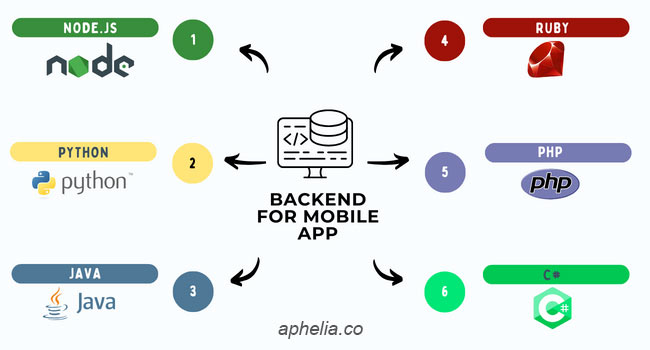
\includegraphics[width=0.75\textwidth]{images/backend_for_mobile_app.jpg}
        \caption{Một số công nghệ phát triển backend cho ứng dụng di động \cite{aphelia2023}.}
        \label{fig:fig1}
      \end{figure}
        \vspace{0.5em}
      
        \hspace*{0.8cm}Về cơ sở dữ liệu, có thể sử dụng các hệ quản trị quan hệ như MySQL hoặc PostgreSQL, tùy theo độ phức tạp của dữ liệu và yêu cầu về hiệu năng. MySQL phù hợp cho các ứng dụng cần tính ổn định cao, trong khi PostgreSQL cung cấp nhiều tính năng nâng cao hơn. Đối với các ứng dụng di động yêu cầu đồng bộ dữ liệu theo thời gian thực, Firebase Firestore là một lựa chọn phù hợp nhờ khả năng cập nhật nhanh và hỗ trợ tốt cho môi trường di động.
      
        \vspace{0.5em}
      
        \hspace*{0.8cm}Phía frontend và mobile, các framework như React Native, Flutter, Swift, và Kotlin là những lựa chọn phổ biến. React Native và Flutter hỗ trợ phát triển ứng dụng đa nền tảng, trong khi Swift và Kotlin là lựa chọn tối ưu cho phát triển ứng dụng gốc trên iOS và Android tương ứng.
      
        \vspace{0.5em}
      
        \hspace*{0.8cm}Cuối cùng, để tăng tính tự động hóa và đảm bảo chất lượng phần mềm, các công cụ CI/CD như GitHub Actions hoặc Jenkins thường được tích hợp vào quy trình phát triển. Bên cạnh đó, việc sử dụng Docker giúp đóng gói và triển khai hệ thống một cách nhất quán trên nhiều môi trường khác nhau.
      
   